%\documentclass[11pt]{amsart}
\documentclass[review]{siamart}
\usepackage{geometry}                % See geometry.pdf to learn the layout options. There are lots.
\geometry{letterpaper}                   % ... or a4paper or a5paper or ... 
%\geometry{landscape}                % Activate for for rotated page geometry
%\usepackage[parfill]{parskip}    % Activate to begin paragraphs with an empty line rather than an indent
\usepackage{graphicx}
\usepackage{amssymb}
\usepackage{epstopdf}
\DeclareGraphicsRule{.tif}{png}{.png}{`convert #1 `dirname #1`/`basename #1 .tif`.png}

\title{Grid/cell services for gyrokinetic particle-in-cell simulations of highly magnetized plasmas}
\author{Mark F. Adams \and Tobin Issac \and Mathew Knepley}
%\date{}                                           % Activate to display a given date or no date
\nolinenumbers
\begin{document}
\maketitle


\begin{abstract} 
The simulation of highly magnetized fusion plasmas presents vast challenges in modeling, discretization, and efficient implementation on emerging architectures.
The Vlasov-Maxwell system is a 6D phase space set of equations and is, more or less, the basis of of all numerical methods in plasma physics.
The gyrokinetic approximation is a common technique to reduce this to a 5D system.
The high dimensionality of this problem lends itself to particle-in-cell (PIC) methods although continuum methods are also used for the whole system or the collision operator.
The dynamics of fusion plasmas is dominated by the strong magnetic guide fields, leading to highly anisotropic models with a large range of time and space scales.
Predictive modeling to be be engineering relevant is one of the great challenged today in computational science.

This document discusses a proposed contribution to this effort: developing fast, both algorithmically efficient and optimized for emerging architectures, continuum grid services for PIC methods for highly magnetized plasmas.
The PETSc project has a great deal of expertise and software for these services (e.g., discretizations, meshing and equation solvers).
This document presents a design of grid, or cell, services, such as Poisson and implicit PIC solvers, gradients, and particle-cell interfaces, for PIC simulations in the PETSc numerical library.
We build on the Solver Integrated Tree-based Adaptive Refinement infrastructure in PETSc to provide services and abstractions useful for extreme-scale PIC applications.
The fundamental computational challenges are outlined and an initial realization of an extreme-scale PIC data model and code is presented.
\end{abstract}

Particle in cell (PIC) methods are effective approaches for discretizing high dimensional physics models in a variety of fields because of their lower cost on high dimensional problems relative to grid or continuum methods.
PIC methods are naturally composed of three types of processing: 1) particle processing, the evolution of the 5D gyrokinetic Vlasov equation for magnetized plasmas, 2) grid processing, and 3) particle-grids interactions.
Most, say well over $99\%$, of the data in a PIC simulation of a fusion devise is in the particles.
This means that the pure grid work, such as the Poisson solver, have abundant computational resources available and, for instance, can be run entirely on the CPU of accelerated architectures, or on a reduced set of cores on symmetric systems.
Note, the collision operator uses a 5D grid solve that is computationally demanding and fast solvers for emerging architectures are required.
Pure particle processing, such as the ``push" of particles is relatively simple array processing.
Particle-grids interactions are very challenging because because the data structures and nature data decompositions are very different.
The physics community has avoided some of this complexity by redundantly storing the entire field data (grid) on each MPI process or address space.
This data model is not tenable as we move to the exa-scale levels of parallelism required for engineering relevant ITER simulations.

The accurate and efficient simulations of these problems to be of engineering relevance, for say the design and operation of ITER, is an extremely challenging problem.
The physics community has developed a large body of research and experience in using PIC methods for fusion plasmas and they are one of the largest users in DOE leader class compute facilities.
The applied math, engineering, computational science, and physics communities have developed a great deal of expertise in discretization and solver methods for extreme-scale computing, but these advanced methods are not widely used in the fusion community.
The continued advancement of fusion simulations within DOE and the global community, especially as we move from reproducing know physics to engineering relevant predictive analysis, requires that both modern numerical methods and modern data decompositions and parallel computing techniques be employed.
These advanced methods require a large amount of engineering investment.
The goal of this work is to amortize these development costs, and the intellectual resources required to develop these algorithms, by developing an integrated solver, discretization, and meshing infrastructure in the widely deployed numerical library PETSc that provides grid services required by PIC codes, such as mesh generation, discretizations, fast equation solvers, gradients and grid deposition at particle positions.
This work builds on the Solver Integrated Tree-based Adaptive Refinement (SITAR) infrastructure in PETSc, which provides fast multigrid equations solvers that are tightly integrated with meshing and discretization of optimal efficiency on emerging architectures.
SITAR is bases on the {\it p4est distributed tree library} \cite{Rudi:2015:EIS:2807591.2807675,DBLP:journals/siamsc/IsaacBWG15}.

\section{Design Requirements}

Parallel grid decompositions
 - deposition-solve-push
 - collisons
 Hierarchical grids for fast geometric multigrid solvers and adaptive mesh refinement
 Abstracting the grid form the physicists so that a variety of grids and discretizations can be used in the same code, often selected at run time with command line parameters. 
 Incremental problems capacity, allowing for debugging and verification on simple grids (e.g., Cartesian grids) to full tokamak wall geometries.
 Fully convergent numerical methods that solve the given PDE with no free parameters other than those that explicitly appear in the equations (e.g., resistivities in resistive MHD).
This requires particle shape factors or density smoothing to allow for arbitrary mesh resolution without increasing particle count to avoid particle noise and allows for code verification with convergence studies.

\section{An Extreme Scale PIC Code for Fusion Plasmas: X2}

\subsection{Uses of X2}

Explore data decompositions and collect performance data to help further refine effective distributed data models for fusion PIC applications.
Cross code verify existing fusion PIC code with simple physics but full ITER wall geometries.

\begin{figure}[h!]
   \centering
   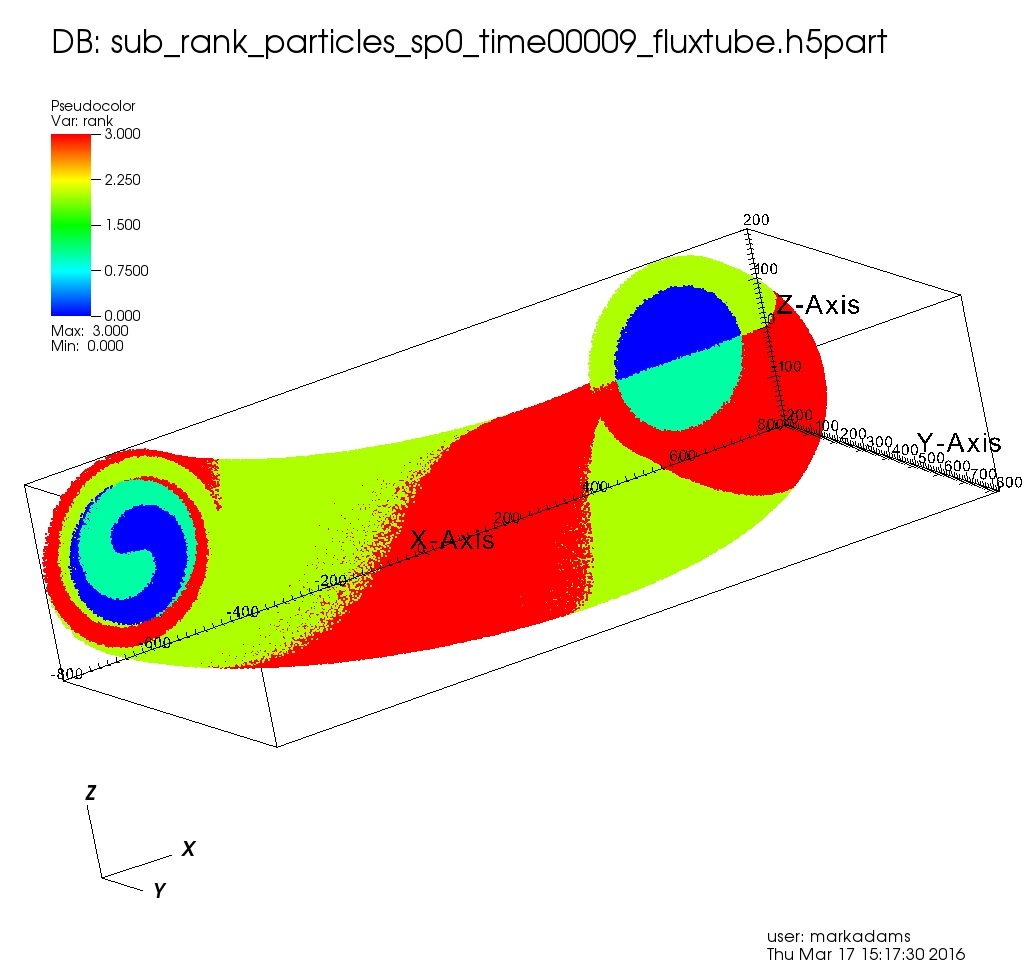
\includegraphics[width=80mm]{half_grid.jpeg} 
   \caption{Particle processor ranks in half the domain of a torus in flux tube data partitions}
   \label{fig:cross}
\end{figure}
 
\begin{figure}[h!]
   \centering
   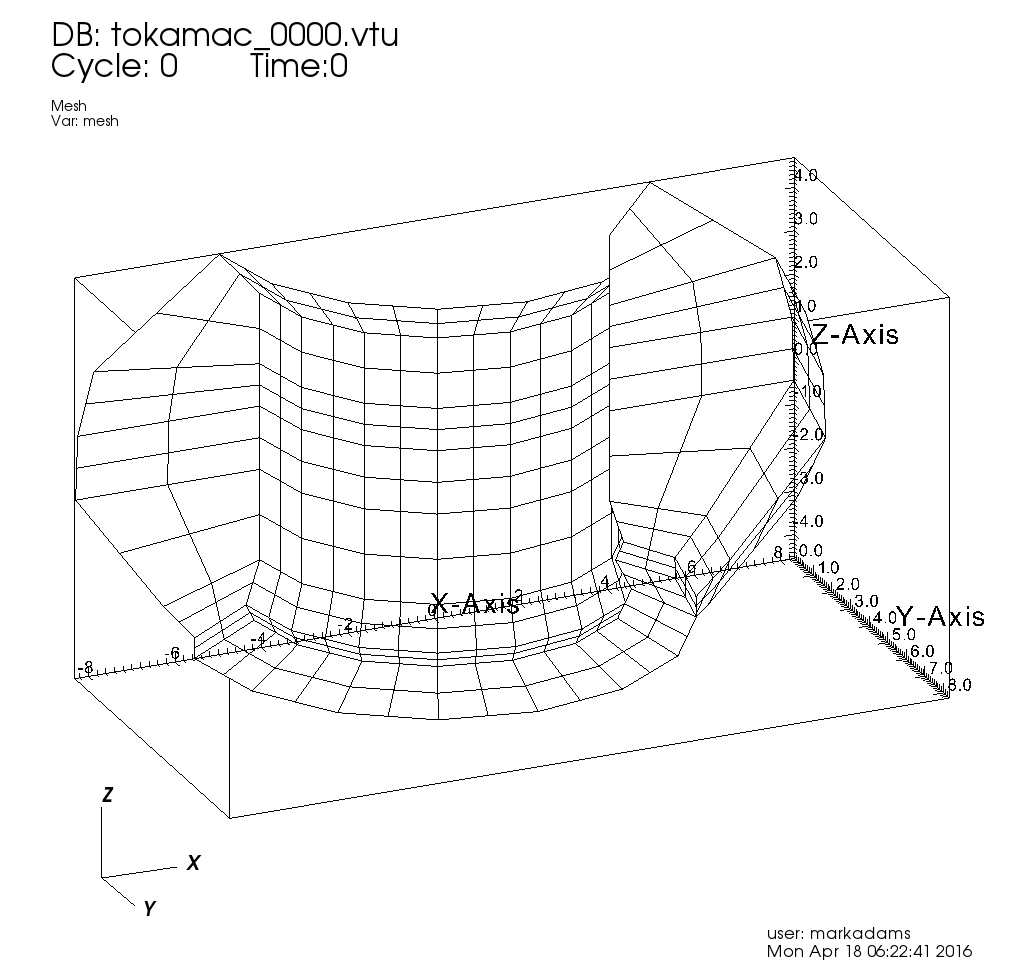
\includegraphics[width=80mm]{half_grid_mesh.jpeg} 
   \caption{Solver grid of half the domain of a torus}
   \label{fig:mesh}
\end{figure}


\bibliographystyle{siamplain}
\bibliography{./bib}


 
\end{document}  